\documentclass[11pt,a4paper]{article}
\usepackage[utf8]{inputenc}
\usepackage[T1]{fontenc}
\usepackage{lmodern}
\usepackage[french]{babel}
\usepackage[margin=2.1cm]{geometry}
\usepackage{microtype}
\usepackage{amsmath,amssymb}
\usepackage{booktabs}
\usepackage{array}
\usepackage[table]{xcolor}
\usepackage{graphicx}
\usepackage{caption}
\usepackage{eurosym}
\usepackage[most]{tcolorbox}
\definecolor{navy}{HTML}{1F3864}
\definecolor{bluemid}{HTML}{2E5496}
\definecolor{lightblue}{HTML}{D6E0F0}
\captionsetup{font=small,labelfont={bf,color=navy},labelsep=period}
\graphicspath{{../figures/}}
\newtcolorbox{cle}[1][]{colback=lightblue!40,colframe=navy,boxrule=0.6pt,
  arc=2pt,left=8pt,right=8pt,top=6pt,bottom=6pt,#1}

\title{\vspace{-1.2cm}\color{navy}\bfseries Benchmark externe\\[2pt]
  \large La plausibilité de l'ordre de grandeur du SCR}
\author{Kélian Kaddouri}
\date{27 juillet 2026}

\begin{document}
\maketitle
\vspace{-0.9cm}

\begin{cle}
\textbf{La question.} \og{}Ce nombre est-il crédible~?\fg{} Le benchmark réglementaire (contre la
Formule Standard, aveugle au risque : charge $\sim$450~M\euro) est déjà au mémoire. Il manque le
contrôle de plausibilité \emph{externe}, face aux pertes et au marché cyber réels.
\end{cle}

\medskip
\begin{center}
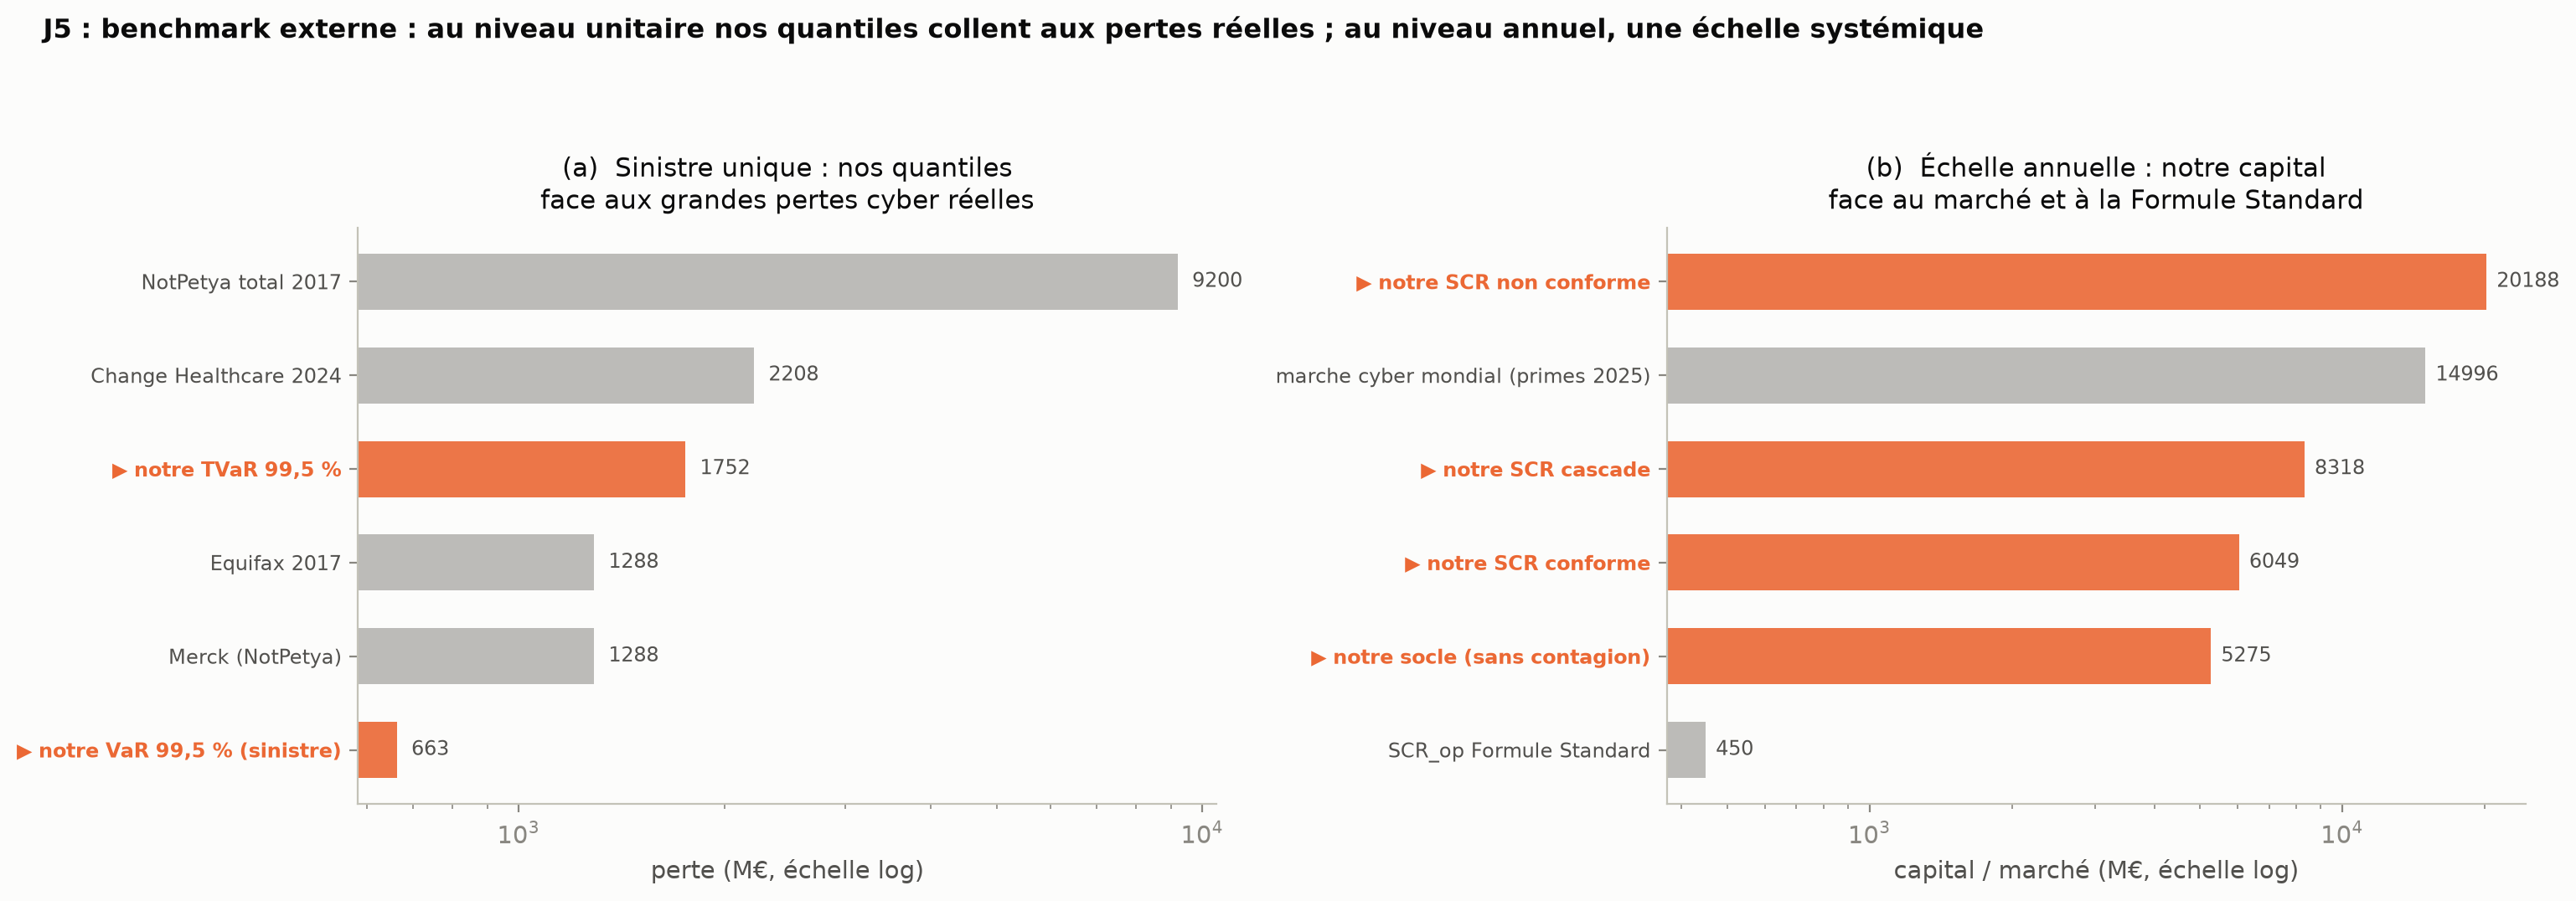
\includegraphics[width=\linewidth]{J5_benchmark_externe.png}
\captionof{figure}{\textbf{(a)} au niveau du sinistre unique, nos quantiles (VaR et TVaR
$99{,}5\,\%$) s'insèrent parmi les grandes pertes cyber réelles. \textbf{(b)} à l'échelle
annuelle, notre capital est d'ordre systémique (comparable au marché mondial) et domine de loin
la charge de la Formule Standard.}
\end{center}

\noindent\textbf{Au niveau du sinistre unique, l'ordre de grandeur est crédible.} Notre VaR
$99{,}5\,\%$ ($663$~M\euro) et notre TVaR ($1\,752$~M\euro) tombent dans la fourchette des
grandes pertes cyber réelles : Merck-NotPetya ($\sim$1,3~Md\euro), Equifax ($\sim$1,3), Change
Healthcare 2024 ($\sim$2,2), sous le choc systémique NotPetya ($\sim$9~Md\euro au total). La
brique de sévérité est bien calibrée à l'échelle de l'événement.

\medskip
\noindent\textbf{Au niveau annuel, c'est une échelle systémique.} Le SCR ($\sim$6 à 20~Md\euro
selon la conformité) est de l'ordre du marché cyber mondial ($\sim$15~Md\euro de primes,
$16{,}3$~Md\$ en 2025). Le périmètre est donc celui d'un \textbf{secteur / grand portefeuille}
(OpRisk financier mondial, $\sim$21,6 incidents matériels par an), non d'une entité moyenne
isolée.

\begin{cle}
\textbf{Verdict.} Le modèle n'est ni \textbf{gonflé} (il colle aux pertes réelles au niveau
unitaire) ni \textbf{aveugle} (il capte, au niveau agrégé, le risque que la Formule Standard
manque). L'ordre de grandeur est crédible, à condition de lire l'agrégat comme un capital de
secteur.
\end{cle}

\smallskip
\noindent\footnotesize\textcolor{navy}{\textbf{Source.}} Script
\texttt{1\_fondations/49\_benchmark\_externe.py}, figure \texttt{J5\_benchmark\_externe.png}.
Repères : marché cyber $16{,}3$~Md\$ GWP 2025 (Business Insurance, III) ; NotPetya, Change
Healthcare, Equifax (presse spécialisée).

\end{document}
